\documentclass[UTF8]{ctexart}
\usepackage{geometry}
\geometry{margin=1.5cm, vmargin={0pt,1cm}}
\setlength{\topmargin}{-1cm}
\setlength{\paperheight}{29.7cm}
\setlength{\textheight}{25.3cm}

% useful packages.
\usepackage{amsfonts}
\usepackage{amsmath}
\usepackage{amssymb}
\usepackage{amsthm}
\usepackage{enumerate}
\usepackage{graphicx}
\usepackage{multicol}
\usepackage{fancyhdr}
\usepackage{layout}
\usepackage{float, caption}
\usepackage{xcolor}
\usepackage{listings}
\usepackage{tikz}

% 自定义配色方案,尽量模仿 VS Code 的高亮效果
\definecolor{codegreen}{rgb}{0,0.6,0}
\definecolor{codeblue}{rgb}{0,0,0.9}
\definecolor{codepurple}{rgb}{0.58,0,0.82}
\definecolor{codered}{rgb}{0.8,0,0}
\definecolor{backcolor}{rgb}{0.95,0.95,0.95}

% lstlisting 的风格设置
\lstdefinestyle{vscode}{
	backgroundcolor=\color{backcolor},   % 背景颜色
	commentstyle=\color{codegreen},     % 注释颜色
	keywordstyle=\color{codeblue}\bfseries, % 关键字颜色
	numberstyle=\tiny\color{gray},      % 行号颜色
	stringstyle=\color{codered},        % 字符串颜色
	basicstyle=\ttfamily\footnotesize,  % 基本字体
	breakatwhitespace=false,            % 仅在空格处断行
	breaklines=true,                    % 自动换行
	captionpos=b,                       % 标题位置(bottom)
	keepspaces=true,                    % 保持空格
	numbers=left,                       % 显示行号
	numbersep=5pt,                      % 行号与代码间的间隔
	rulecolor=\color{black},            % 框线颜色
	showspaces=false,                   % 不显示空格符号
	showstringspaces=false,             % 不显示字符串中的空格
	showtabs=false,                     % 不显示制表符
	frame=single,                       % 外框
	tabsize=4,                          % 制表符宽度
	escapeinside={(*@}{@*)},            % 特殊字符转义
	morekeywords={*,...}                % 添加更多自定义关键字
}
\lstset{style=vscode}

% some common command
\newcommand{\dif}{\mathrm{d}}
\newcommand{\avg}[1]{\left\langle #1 \right\rangle}
\newcommand{\difFrac}[2]{\frac{\dif #1}{\dif #2}}
\newcommand{\pdfFrac}[2]{\frac{\partial #1}{\partial #2}}
\newcommand{\OFL}{\mathrm{OFL}}
\newcommand{\UFL}{\mathrm{UFL}}
\newcommand{\fl}{\mathrm{fl}}
\newcommand{\op}{\odot}
\newcommand{\Eabs}{E_{\mathrm{abs}}}
\newcommand{\Erel}{E_{\mathrm{rel}}}

\lstdefinestyle{json}{
	basicstyle=\ttfamily\footnotesize,
	commentstyle=\color{gray},
	stringstyle=\color{red},
	keywordstyle=\color{blue},
	numbers=left,
	numberstyle=\tiny\color{gray},
	stepnumber=1,
	numbersep=5pt,
	backgroundcolor=\color{white},
	showspaces=false,
	showstringspaces=false,
	showtabs=false,
	tabsize=2,
	breaklines=true,
	frame=single,
	captionpos=b
}
\begin{document}
	
	\pagestyle{fancy}
	\fancyhead{}
	\lhead{高凌溪, 3210105373}
	\chead{微分方程数值解project \#1报告}
	\rhead{\today}
	\begin{abstract}
		本次编程作业实现了多重网格求解线性方程组$Ax=b$,其中$A$是一维Poission方程或二维Poission方程离散的矩阵。
	\end{abstract}
	\section{程序设计原理和思路}
	\subsection{限制算子}
		一维时,限制算子应该是$\mathbb{R}^{n+1} \to \mathbb{R}^{\frac{n}{2}+1}$的一个线性算子;二维时,限制算子是$\mathbb{R}^{(n+1)(n+1)} \to \mathbb{R}^{(\frac{n}{2}+1)(\frac{n}{2}+1)}$的一个线性算子。\\
		设向量$v=(v_0, v_1,...,v_{n})$,则
	\subsubsection{injection 算子}
	\begin{itemize}
		\item 对于一维的情况,按照讲义给出的方法,定义$v^{2h}_j=v^h_{2j}, j=0,1,...,\frac{n}{2}$。
		\item 对于二维的情况,仍然是将细网格的值限制在粗网格上,此时用指标$(i,j)$来代表行列的编号,有$v^{2h}_{(i,j)}=v^h_{2i, 2j}$,\\
		这里$j=0,1,...\frac{n}{2}, \quad i=0,1,...,\frac{n}{2}$
	\end{itemize}
	\subsubsection{full-weighting算子}
	\begin{itemize}
		\item 对于一维的情况,按照讲义给出的方法,定义$v^{2h}_{j}=\frac{1}{4}v^h_{2j-1}+\frac{1}{2}v^h_{2j}+\frac{1}{4}v^h_{2j+1},\quad j=1,...,\frac{n}{2}-1$。对于端点上的值,仍然直接使用injection的方法。
		\item 对于二维的情况,使用krocker积,此时将权重看成一个向量$v=\left(\frac{1}{4},\frac{1}{2}, \frac{1}{4}\right)$,那么此时用9个点平均粗网格上的值,系数矩阵应该为:$v^T\otimes v$,即\\
		$v^{2h}_{(i,j)}=\frac{1}{16}v^h_{(2i-1,2j-1)}+\frac{1}{8}v^h_{(2i,2j-1)}+\frac{1}{16}v^h_{(2i+1, 2j-1)}+\frac{1}{8}v^h_{(2i-1,2j)}+\frac{1}{4}v^h_{(2i,2j)}+\frac{1}{8}v^h_{(2i+1,2j)}+\frac{1}{16}v^h_{(2i-1,2j+2)}+\frac{1}{8}v^h_{(2i,2j+1)}+\frac{1}{16}v^h_{(2i+1,2j+1)}$
	\end{itemize}
	\subsection{插值算子}
		一维时,插值算子应该是$\mathbb{R}^{\frac{n}{2}+1} \to \mathbb{R}^{n+1}  $的一个线性算子;二维时,插值算子是$\mathbb{R}^{(\frac{n}{2}+1)(\frac{n}{2}+1)} \to \mathbb{R}^{(n+1)(n+1)}$的一个线性算子。\\
		设向量$v=(v_0, v_1,...,v_{n-1})$。
	\subsubsection{线性插值}
	\begin{itemize}
		\item 一维时线性插值按照讲义上的公式,对于细网格边界旁边的点(下图中黑色的点)有:
		\begin{center}
			\begin{tikzpicture}
				
				% 低层插值点 (T_{J-1})
				\foreach \x in {0,2,4,6,8}
				\filldraw[blue] (\x,0) circle (3pt);
				\draw (0,0) -- (8,0);
				\node[right] at (8.5,0) {\Large $v^{2h}$};
				
				% 高层插值点 (T_J)
				\foreach \x in {0,1,2,3,4,5,6,7,8} {
					\ifnum\x=1
					\filldraw[black] (\x,1.5) circle (3pt);
					\else
					\ifnum\x=7
					\filldraw[black] (\x,1.5) circle (3pt);
					\else
					\ifodd\x
					\filldraw[red] (\x,1.5) circle (3pt);
					\else
					\filldraw[blue] (\x,1.5) circle (3pt);
					\fi
					\fi
					\fi
				}
				\draw (0,1.5) -- (8,1.5);
				\node[right] at (8.5,1.5) {\Large $v^h$};
				
			\end{tikzpicture}
		\end{center}
		对于粗网格上的点,直接保留\\
		$v^{2h}_{2j}=v^h_j\quad j=0,1,...,\frac{n}{2}$
		对于内部的细网格点,有\\
		$v^h_{2j+1}=\frac{1}{2}v^{2h}_{j}+\frac{1}{2}v^{2h}_{j+1}\quad j=0,1,2,...,\frac{n}{2}-1$\\
		$v^h_{2j-1}=v^{2h}_{j-1}\quad j=1,2,...,\frac{n}{2}-1$
		\item 对于二维的情况,我们的点可以分成下面的几类:
		\begin{center}
			\begin{tikzpicture}
								% 颜色列表
				\definecolor{myblue}{RGB}{0,114,178}
				\definecolor{myyellow}{RGB}{240,228,66}
				\definecolor{mygreen}{RGB}{0,158,115}
				\definecolor{mypurple}{RGB}{204,121,167}
				\definecolor{myorange}{RGB}{230,159,0}
				% 左侧粗网格
				\draw[thin] (0,0) grid (4,4);
				
				% 插值点(蓝色)
				\foreach \x in {1,2,3}
				\foreach \y in {1,2,3}
				\filldraw[myblue] (\x,\y) circle (2pt);
				
				% 右侧细网格
				\draw[thin] (6,0) grid (10,4);
				\draw[thin] (6,0) grid[step=0.5] (10,4); % 细网格
				
				% 右侧网格插值点(不同颜色)
				\foreach \x in {7,8,9}
				\foreach \y in {1,2,3} 
				\filldraw[myblue] (\x,\y) circle (2pt);
				
				\foreach \x in {7.5,8.5}
				\foreach \y in {1.5, 2.5}
				\filldraw[myyellow] (\x,\y) circle (2pt);
				
				\foreach \x in {7.5,8.5}
				\foreach \y in {1,2,3}
				\filldraw[mypurple] (\x,\y) circle (2pt);
				
				\foreach \x in {7,8,9}
				\foreach \y in {1.5,2.5}
				\filldraw[mypurple] (\x,\y) circle (2pt);
				
			\end{tikzpicture}
		\end{center}
		参考William L.Briggs的A Multigrid Tutoral,有下面的插值格式
		\[v_{2i,2j}^h = v_{ij}^{2h},\]
		
		\[v_{2i+1,2j}^h = \frac{1}{2}(v_{ij}^{2h} + v_{i+1,j}^{2h}),\]
		
		\[v_{2i,2j+1}^h = \frac{1}{2}(v_{ij}^{2h} + v_{i,j+1}^{2h}),\]
		
		\[v_{2i+1,2j+1}^h = \frac{1}{4}(v_{ij}^{2h} + v_{i+1,j}^{2h} + v_{i,j+1}^{2h} + v_{i+1,j+1}^{2h}),\quad 0 \leq i,j \leq \frac{n}{2}-1.\]
		对于蓝色的粗网格上的点,我们直接用粗网格的值;对于紫色的点,用一维的插值去平均;对于黄色的点,用周围四个蓝色的点去平均;
	\end{itemize}
	\subsubsection{二次插值}
	\begin{itemize}
		\item 对于一维的情况,
				\begin{center}
			\begin{tikzpicture}
				
				% 低层插值点 (T_{J-1})
				\foreach \x in {0,2,4,6,8}
				\filldraw[blue] (\x,0) circle (3pt);
				\draw (0,0) -- (8,0);
				\node[right] at (8.5,0) {\Large $v^{2h}$};
				
				% 高层插值点 (T_J)
				\foreach \x in {0,1,2,3,4,5,6,7,8} {
					\ifnum\x=1
					\filldraw[black] (\x,1.5) circle (3pt);
					\else
					\ifnum\x=7
					\filldraw[black] (\x,1.5) circle (3pt);
					\else
					\ifodd\x
					\filldraw[red] (\x,1.5) circle (3pt);
					\else
					\filldraw[blue] (\x,1.5) circle (3pt);
					\fi
					\fi
					\fi
				}
				\draw (0,1.5) -- (8,1.5);
				\node[right] at (8.5,1.5) {\Large $v^h$};
				
			\end{tikzpicture}
		\end{center}
		对黑色的点用三个点插值,红色的点用四个点插值,可以得到:\\
		\[
		v^h_0=\frac{3}{8}v^{2h}_0+\frac{6}{8}v^{2h}_1-\frac{1}{8}v^{2h}_2 \quad v^h_{n}=\frac{6}{8}v^{2h}_{\frac{n}{2}-2}+\frac{6}{8}v^{2h}_{\frac{n}{2}-1}-\frac{1}{8}v^{2h}_{\frac{n}{2}}
		\]
		\[
		v^{h}_{2j}=v^{2h}_j\quad j=0,1,...,\frac{n}{2}-2
		\]
		\[
		v^{h}_{2j+1}=\frac{9}{16}v^{2h}_j+\frac{9}{16}v^{2h}_{j+1}-\frac{1}{16}v^{2h}_{j+2}-\frac{1}{16}v^{2h}_{j-1}
		\]
		\item 对于二维的情况:\\
			\begin{center}
			\begin{tikzpicture}
				% 颜色列表
				\definecolor{myblue}{RGB}{0,114,178}
				\definecolor{myyellow}{RGB}{240,228,66}
				\definecolor{mygreen}{RGB}{0,158,115}
				\definecolor{mypurple}{RGB}{204,121,167}
				\definecolor{myorange}{RGB}{230,159,0}
				% 左侧粗网格
				\draw[thin] (0,0) grid (4,4);
			
				
				\filldraw[myyellow] (1.5,1.5) circle (2pt);
				
				\foreach \x in {0,1,2,3}
				\foreach \y in {0,1,2,3}
				\filldraw[mygreen] (\x,\y) circle (2pt);
				
				
				% 右侧细网格
				\draw[thin] (6,0) grid (10,4);
				\draw[thin] (6,0) grid[step=0.5] (10,4); % 细网格
				
				% 右侧网格插值点(不同颜色)
				\foreach \x in {7,8,9}
				\foreach \y in {1,2,3} 
				\filldraw[myblue] (\x,\y) circle (2pt);
				
				
				\foreach \x in {7.5,8.5}
				\foreach \y in {1.5, 2.5}
				\filldraw[myyellow] (\x,\y) circle (2pt);
				
				\foreach \x in {7.5,8.5}
				\foreach \y in {1,2,3}
				\filldraw[mypurple] (\x,\y) circle (2pt);
				
				\foreach \x in {7,8,9}
				\foreach \y in {1.5,2.5}
				\filldraw[mypurple] (\x,\y) circle (2pt);
				
				\foreach \x in {6.5,7,7.5,8,8.5,9,9.5}
				\foreach \y in {0.5, 3.5}
				\filldraw[myorange] (\x,\y) circle (2pt);
				
				\foreach \x in {6.5,9.5}
				\foreach \y in {0.5,1,1.5,2,2.5,3, 3.5}
				\filldraw[myorange] (\x,\y) circle (2pt);
				
			\end{tikzpicture}
		\end{center}
		对于蓝色的点,直接使用粗网格上的值即可;对于紫色的点,使用一维的二次插值;对于橙色的点,令$v=v=\left(\frac{-1}{16}, \frac{9}{16}, \frac{9}{16}, \frac{-1}{16}\right),\ u=\left(\frac{3}{8},\frac{6}{8}, \frac{-1}{8}\right)$,则插值格式应为$v^T \otimes u$;对于右图中黄色的点,由于一维时的插值格式是$v=\left(\frac{-1}{16}, \frac{9}{16}, \frac{9}{16}, \frac{-1}{16}\right)$,相应的选择二维的插值格式是$v^T \otimes  v$用左图中的16个点插值,

	\end{itemize}
	\section{拉普拉斯算子的离散}
	\begin{itemize}
		\item \textbf{Dirichlet边界:}直接离散。
		\item \textbf{Neumann边界:}在边界上利用ghost cell逼近导数,然后在边界上求离散拉普拉斯算子。此时离散出来的矩阵不可逆,在做w\_Jacobi迭代时,每次都取与零空间正交的解,最后在加上相差的常数。
		\item \textbf{Mixed边界条件:}二维时为了避免正方形四个角上定义冲突,直接给出解在四个角上的值。
	\end{itemize}
	\section{粗网格上的求解和Relaxation中权重的选择}
	\subsection{Relaxation中权重的选择}
	\begin{itemize}
		\item \textbf{一维情况:}对于Dirichlet边界,离散得到的矩阵对称正定,此时特征值设为$\lambda_k,\quad k=1,2,...,n+1$,其中$k_1=k_2=2$,其余的特征值课本已经给出,选择松弛因子$\omega=\frac{2}{3}$。对于其他边界条件,离散出来的矩阵不对称,但是仍然选择$\omega=\frac{2}{3}$作为松弛因子。
		\item \textbf{二维情况:}选择 $\omega=\frac{4}{5}$作为松弛因子。
	\end{itemize}
	
	\section{结果分析}
	所有的结果都保存在output文件夹中,在\texttt{json}文件中,我输出了误差向量的1-范数、2-范数、无穷范数和迭代次数,在\texttt{csv}文件中我输出了每次求解的运行时间。\\
	设置当迭代次数大于用户给出的最大迭代次数或者当$\left \| x_{k+1}-x_k \right \|_2 < \epsilon$时,停止迭代。这里$x_{k+1}$表示第$k+1$次迭代得到的解。\\
	可以发现一次插值的稳定性比二次插值要好。当网格很大时,二次插值对Neumann边值问题得到的解发散。对Mixed边界条件,得到的解误差也不如Dirichlet问题精确。且当网格为$256$时,求解速度明显很慢,已经接近$3000 ms$。
\end{document}
